\documentclass[a4paper, 12pt]{article}
\usepackage[utf8]{inputenc}
\usepackage[french]{babel}
\usepackage[T1]{fontenc}
\usepackage[top=2cm, bottom=2cm, left=2cm, right=2cm]{geometry}
\usepackage{graphicx}
\usepackage{listings}
\usepackage{xcolor}
\usepackage{hyperref}
\usepackage{amsmath, amssymb}
\usepackage{enumitem}
\usepackage[justification=centering]{caption}

\date{Mai 2020}

\begin{document}
\definecolor{commentgreen}{RGB}{2,112,10}
\definecolor{eminence}{RGB}{108,48,130}
\definecolor{weborange}{RGB}{255,165,0}
\definecolor{frenchplum}{RGB}{129,20,83}
\lstset{language=C,
  frame=tb,
  tabsize=4,
  showstringspaces=false,
  commentstyle=\color{commentgreen},
  keywordstyle=\color{eminence},
  stringstyle=\color{red},
  basicstyle=\small\ttfamily,
  emph={int,char,double,float,unsigned,void,bool},
  emphstyle={\color{blue}},
  escapechar=\&,
  classoffset=1,
  otherkeywords={>,<,.,;,-,!,=,~},
  morekeywords={>,<,.,;,-,!,=,~},
  keywordstyle=\color{weborange},
  classoffset=0,
}
\renewcommand{\lstlistingname}{Programme}
\thispagestyle{empty}

\vfill
\begin{center}
  \vspace*{1.5cm}
  \LARGE Projet de programmation impérative - Semestre 6\\[1cm]
  \Large Filière Informatique\\[2cm]
  {\Huge \bfseries Hex\\[0.4cm]}
  \rule{\linewidth}{0.1cm}\\[2cm]
  {\Large Antoine CHARTRON \quad David GOND \\\quad Hamza BENMENDIL \quad Mehdi BEN SALAH}\\[0.5cm]
  \Large Groupe 9150 \\[1cm]
  \Large Année 2019-2020 \\ [3cm]
  
\includegraphics[width=0.3\textwidth]{./pictures/logo.png}\\[0.5cm]
  \LARGE \bsc{Enseirb-Matmeca}\\[1.5cm]
  \vfill

\end{center}

\newpage
\thispagestyle{empty}
\section*{Remerciements}
Nous tenons à remercier toutes les personnes qui ont contribué au développement du projet, qui nous ont aidés et conseillés.
Tout d'abord, nous adressons nos remerciements à notre encadrant, M. Herbreteau, pour sa bienveillance et son aide dans de nombreuses parties du projet.

Nous remercions également M. Renault, pour son encadrement et son aide dans les différentes problématiques rencontrées.
\newpage
\tableofcontents
\setcounter{page}{1}
\newpage

\section{Présentation du sujet}
Ce projet du semestre 6 avait pour thème le jeu de société Hex. Il se joue originellement à 2 joueurs sur un plateau à cases hexagonales. Chaque joueur se voit attribuer une couleur, leur but étant, de relier deux bords opposés du plateau avec des cases de leur propre couleur. Les joueurs jouent une case chacun leur tour. Le sujet apporte quelques modifications au jeu d'origine, puisque la taille et le format du plateau sont paramétrables.

Dans un premier temps, l'objectif du projet était de permettre à des joueurs avec des stratégies différentes de jouer une partie de Hex. Pour cela, il fallait donc un serveur de jeu et des joueurs. Dans un second temps, le but était de développer des stratégies de jeu, en se servant notamment de l'article du mathématicien et informaticien Anshelevich, afin d'obtenir la gloire d'être premier du classement. Un point important est la compatibilité de notre code avec celui des autres équipes. Pour pouvoir faire jouer les stratégies les unes contre les autres, elles devaient partager des interfaces similaires.

\section{Organisation de l'équipe}
L'organisation est un élément central dans un projet en équipe, afin de se coordonner et de s'entendre sur la conception et les solutions à mettre en place. Cela permet de passer outre les écueils habituels d'un tel projet et de gagner un temps précieux. De plus, au vu des conditions exceptionnelles dans lesquelles se sont déroulées ce projet, la communication jouait un rôle primordiale dans le bon déroulement de ce dernier.

\subsection{Répartition des tâches}
Afin de mieux identifier les différentes problématiques auxquelles nous allions être confrontés et de comprendre le fonctionnement global du programme que nous allions devoir implémenter, nous avions réalisé un découpage en tâches. Le site web Taiga\footnote{Taiga est un site web qui permet la gestion de projets grâce aux méthodes agiles Scrum et Kanban.} nous a permis de créer nos tâches et de les disposer facilement dans un tableau Kanban\footnote{Un tableau Kanban est constitué de plusieurs colonnes dans lesquelles il est possible de déplacer une note afin d'indiquer son état d'avancement.}. L'avantage est qu'il est facilement possible de rajouter des nouvelles tâches lors du développement si un nouveau problème est soulevé par le sujet ou bien un membre de l'équipe. Il permet également de voir très rapidement l'avancement du projet ainsi que les tâches effectuées par les coéquipiers.

\subsection{Communication}
Comme expliqué ci-dessus, la communication a été très importante durant toute la durée du projet. Pour rester en contact avec nos encadrants, qui nous fournissaient aide et renseignements, nous avons utilisé Slack. Du côté de l'équipe nous communiquions principalement sur un serveur Discord dédié à nos deux projets du semestre 6. Il nous a ainsi été simple de communiquer via messages ou conversations audio, et ce, tout au long du projet.

\subsection{Utilisation de Git}
Git est un outil dont nous connaissions les bases. Pour simplifier le développement et éviter le plus possible des conflits chronophages, nous avons choisi d'utiliser des branches. Cela a pour avantage de découper clairement les tâches en cours de réalisation dans des branches différentes, mais nous permet également de pouvoir identifier et gérer plus facilement les sources d'un potentiel problème. Le principal désavantage est qu'il n'est pas possible de savoir si la forge valide cette branche.

\section{Conception}
Cette partie va s'intéresser au travail préparatoire ayant été réalisé avant l'écriture d'un quelconque code. La conception permet de comprendre les différents enjeux du projet et d'anticiper les problématiques.

\subsection{Organisation des fichiers et compilation}
L'étude des fonctionnements demandés et des détails techniques imposés pour la mise en place du projet, fut une étape importante. C'est des différentes contraintes et nécessité que l'architecture globale du programme a été obtenu.

\subsubsection{Organisation des fichiers.}
L'interopérabilité étant un point important du sujet, il était nécessaire de respecter les interfaces déjà fournies. Cependant, certaines fonctionnalités semblaient avoir besoin d'être dans des fichiers non référencés par le sujet. Par exemple les fichiers qui permettent de charger dynamiquement un joueur et qui sont discutés dans la partie \ref{spart:j}, sont indispensables mais pas mentionnés. La figure \ref{fig:dep}, ci-dessous, montre les inclusions nécessaires à chacun des fichiers. Il permet d'identifier facilement les dépendances entre fichiers et donc d'éviter les interdépendances. Il montre également l'architecture globale du programme qui permet une meilleure mise en place des règles de compilation.

\begin{figure}[h]
  \centering
  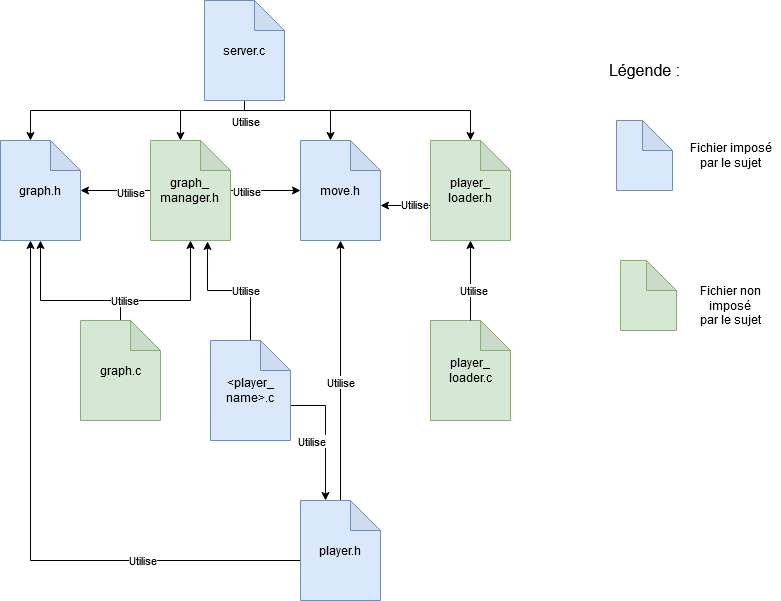
\includegraphics[width=.9\linewidth]{./pictures/dependencie.png}
  \caption{Schéma des dépendances des fichiers.}
  \label{fig:dep}
\end{figure}

\subsubsection{Compilation}
Le projet demandant la création de plusieurs exécutables et stratégies, nous avons dû mettre en place une organisation claire des fichiers et une uniformisation des compilations des stratégies. Afin de pratiquer un des modules du semestre, nous avons mis en place une organisation de fichiers propice à une utilisation de \emph{Cmake}.  En séparant les fichiers sources des fichiers de tests, en configurant les créations des exécutables \emph{server} et \emph{alltests} ainsi que les stratégies en librairies partagées nous avons créé cet environnement favorable. Puisque la forge effectuait des commandes \emph{make} pour exécuter les tests et vérifications telle que \emph{valgrind}, nous avons créé une configuration \emph{Makefile} qui met en place l'environnement de build et lance les commandes de \emph{Cmake}. Cette configuration permettait non seulement à notre projet de fonctionner sur la forge, mais également d'ajouter des commandes supplémentaires, comme par exemple la compilation séparée de la bibliothèque de tests \emph{Cyounit}, qui ne dépendait pas du projet et qui possédait déjà sa propre configuration \emph{Cmake}.

Un autre avantage à l'utilisation de \emph{Cmake} est qu'il existe une commande \emph{find\_package} permettant de trouver une librairie installée sur le système, ce qui nous a été très utile puisque le lien vers la libraire \emph{GSL} sur les machines de l'école et sur, par exemple, Ubuntu n'était pas le même que celui précisé sur le sujet. Celui-ci demandait à pouvoir spécifier un chemin de dossier contenant la libraire, dont les headers se situant dans un sous-dossier \emph{include} et les librairies dans \emph{bin}. Sur les autres systèmes que nous avons utilisés, ces sous-dossiers n'appartenant pas au même dossier parent, il nous était impossible de fournir la librairie en un seul chemin. Cette configuration de \emph{cmake} nous a finalement permis d'utiliser la librairie GSL déjà installée tout en permettant de spécifier un autre chemin si besoin, ce qui n'aurait pas été aussi facile avec uniquement un \emph{Makefile}.

\subsubsection{Exécution du programme}
\label{part:opt}
Afin d'exécuter le programme, il faut fournir au serveur deux clients compilés sous la forme de bibliothèque partagée. Mais il est également demandé de gérer des options qui permettent le paramétrage du plateau de jeu. Il y a ainsi deux options :
\begin{itemize}[label=\textbullet]
\item \texttt{-m} qui permet de spécifier la taille du plateau et qui accepte donc un nombre entier positif strictement supérieur à 1.
\item \texttt{-t} qui permet de spécifier le type de plateau parmi trois différents. Ainsi avec \texttt{-t t} ce sera un plateau triangulaire, avec \texttt{-t h} il sera hexagonal et avec \texttt{-t c} il sera carré.
\end{itemize}

Pour récupérer les options, un parser a été créé. Il affiche également une aide à l'exécution pour indiquer l'erreur commise et la syntaxe de la ligne d'exécution.

\subsection{Conception des joueurs}
\label{spart:j}
Les joueurs sont très importants dans ce projet. Ils implémentent différentes stratégies plus ou moins avancées qui vont s'affronter pour gagner une partie. Mais avant d'étudier les façons de jouer, il était nécessaire de s'intéresser à l'architecture dont un joueur a besoin.
\subsubsection{Restrictions sur les joueurs}
Tout d'abord, plusieurs restrictions étaient imposées par le sujet. Les joueurs étaient considérés comme des clients qui implémentaient une interface commune, permettant ainsi de faire jouer n'importe quel client sur un serveur. Ils possédaient donc tous les mêmes prototypes de fonctions, mais le fonctionnement interne différait d'un joueur à l'autre. Toujours dans un souci d'interopérabilité, chaque client devait être compilé sous la forme de bibliothèque partagée. Ils devaient également être automatiques, c'est-à-dire qu'ils ne nécessitaient aucune intervention extérieure autre que celle du serveur.

Comme les joueurs étaient compilés dans des bibliothèques partagées, il était nécessaire de les charger dynamiquement grâce à la bibliothèque DL.

\subsubsection{Chargement dynamique des joueurs}
Le but du chargement dynamique, via la bibliothèque DL, était de pouvoir définir le comportement du serveur totalement indépendamment des stratégies utilisées, afin de permettre le changement à chaque exécution. Pour cela, il nous a fallu retrouver les éléments communs à toutes les stratégies, en nous servant de leur interface. Nous avons donc remarqué que seules les fonctions communes à tous les joueurs étaient vraiment utiles au serveur. Il est également nécessaire de garder en mémoire le \textit{handler}, qui est retourné par l'ouverture du fichier d'un joueur et qui permet sa fermeture. Nous en avons donc déduit une structure \texttt{player} contenant sept pointeurs de fonctions et un pointeur correspondant au \textit{handler}. Le code \ref{algo:player} correspond à cette structure.

\begin{lstlisting}[language=C, frame=single,columns=fullflexible, breaklines=true, label={algo:player}, mathescape, caption={Implémentation de la structure \texttt{player}.}, captionpos=b]
  /**
  * \struct player
  * \brief The structure represents a player
  * It contains the different functions of the player and the handler
  * to open its library.
  */
  struct player {
    void* handler;
    char const* (*get_player_name)(void);
    struct move_t (*propose_opening)(void);
    int (*accept_opening)(const struct move_t);
    void (*initialize_graph)(struct graph_t*);
    void (*initialize_color)(enum color_t);
    struct move_t (*play)(struct move_t);
    void (*finalize)(void);
  };
\end{lstlisting}

\subsection{Représentation du plateau de jeu}
Le plateau est représenté sous la forme d'un graphe. Les cases sont représentées par les sommets du graphe, deux sommets sont liés d'une arête lorsqu'ils sont adjacents sur le plateau. Ainsi la figure \ref{fig:graphrep}, montre la représentation d'un plateau hexagonale de largeur 3 ainsi que sa représentation sous forme de graphe.

\begin{figure}[h]
  \centering
  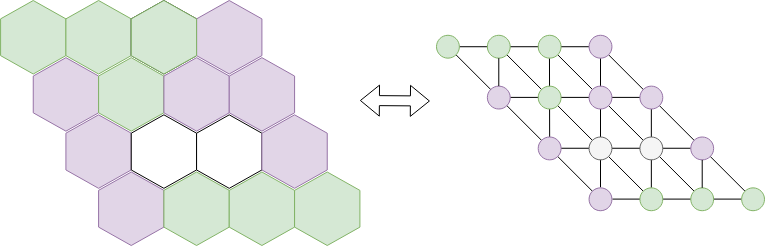
\includegraphics[width=.7\linewidth]{./pictures/graphrep.png}
  \caption{Représentation d'un plateau sous forme de graphe}
  \label{fig:graphrep}
\end{figure}

Ces graphes sont implémentés sous la forme d'une matrice. C'est une matrice d'adjacence qui permet de savoir si deux sommets sont voisins. L'élément de la matrice $(i,j)$ a pour valeur 1 si les sommets $i$ et $j$ sont liés d'une arête, 0 sinon.

Le type de graphes qui représente ce genre de plateaux de jeu donne une matrice où seulement quelques éléments sont non nuls, on utilise pour cela la bibliothèque \emph{GSL} qui fournit plusieurs implémentations du type matrice creuse. Celles-ci permettent d'économiser de la mémoire ainsi que du temps de parcours comparé aux implémentations classiques. L'implémentation qu'on utilise stocke seulement les valeurs non nulles de la matrice sous la forme de triplets $(i,j,valeur)$.

Même si le graphe est représenté, il est nécessaire d'ajouter une autre matrice qui stockera la couleur de chaque sommet. Il s'agit simplement d'une matrice de la taille $(2, n)$, avec $n$ le nombre de sommet.\\

Une fois notre conception et architecture définie, nous avons pu commencer à nous intéresser plus précisément à l'écriture des algorithmes qui allaient réaliser nos besoins.


\section{Solutions algorithmiques}
Cette partie va traiter des différentes solutions algorithmiques survenues au cours de l'écriture du code des clients et des serveurs.

\subsection{Serveur de jeu}
Un serveur est nécessaire pour réguler le jeu. C'est en effet celui-ci qui chargera les joueurs, initialisera le jeu, puis les fera jouer les joueurs un par un. Il permet aussi la détection d'un gagnant ou d'un match \texttt{ex-aequo}.

\subsubsection{Initialisation du jeu}
La première action du serveur est de paramétrer le jeu en entier. Dans un premier temps on utilise le parser pour obtenir les différentes options passées en ligne de commande. Cela permet d'initialiser des variables importantes comme la largeur et le type de plateau. Les options sont expliquées de façons plus exhaustives dans la partie \ref{part:opt}.

Le graphe peut alors être initialisé. Cette opération se réalise en temps polynomial, $\mathcal{O}(m^2)$, où $m$ est la taille du côté du plateau de jeu.

Par la suite, ce sont les joueurs qui sont initialisés grâce aux fonctions réalisant le chargement des joueurs. Intervient alors la \emph{pie rule} pour déterminer la couleur des joueurs et l'ordre de jeu. La complexité de ce fonctionnement est plus compliquée à déterminé car cela dépend entièrement de la stratégie appliquée par le joueur dans ce cas. Cela peut très bien se faire en temps constant, en refusant toujours le premier coup proposé par exemple, ou bien dans un temps bien plus élevé, comme lorsqu'un joueur va évaluer la situation et l'intérêt de la position jouée.

Tout est prêt pour jouer, alors la boucle principale peut maintenant faire jouer les différents joueurs l'un après l'autre.

\subsubsection{Boucle principale}
La boucle principale possède un fonctionnement relativement simple. Tant qu'il n'y a pas de gagnant et qu'il est toujours possible de jouer alors on fait jouer les joueurs tour à tour. Pour ce faire, nous avons placé les deux joueurs dans un tableau. \`A chaque itération l'index est incrémenté et modulé par 2. Cela permet d'appeler la fonction \texttt{play} du bon joueur à chaque tour. Il est aussi à noter que chaque joueur ainsi que le serveur, stocke son propre graphe. Cette sécurité permet de prévenir une potentielle triche provenant des joueurs. \`A chaque itération le plateau du serveur est donc mis à jour.

\subsubsection{Vérification du vainqueur}
Comme spécifié dans le paragraphe précédent, la boucle principale n'est quittée que lorsqu'un gagnant ou un match nul est détecté. Pour détecter un gagnant, nous vérifions, en faisant un parcours simple, s'il existe un chemin allant d'un bord au bord opposé du plateau. Si le retour est négatif, il est indispensable de vérifier que le prochain joueur peut encore jouer. En d'autres termes que nous ne sommes pas en face d'une situation d'\textit{ex-aequo}. Cela se vérifie facilement en parcourant la matrice représentant le plateau. Dès qu'une case n'est attribuée à aucun des deux joueurs, alors il est encore possible de jouer. Le serveur étant prêt, il est temps d'introduire la première stratégie.

\subsection{Le premier joueur}
Afin de faire fonctionner au plus vite notre programme, nous avons choisi d'implémenter la plus simple des stratégies : le choix aléatoire. Même si l'emplacement choisi pour jouer par la stratégie est choisi aléatoirement, des règles doivent être respectées. Il faut notamment que le joueur joue un coup de sa propre couleur, que la position choisie soit comprise dans le graphe représentant le plateau et enfin que la position choisie n'est pas déjà été choisi au préalable. La connaissance des emplacements libres est primordiale dans le choix d'un nouvel emplacement où jouer. Pour stocker ces sommets libres, il nous a semblé nécessaire d'utiliser un type abstrait de donnée : l'ensemble.

\subsection{TAD ensemble}
Ce type abstrait de donnée a été réalisé lors du cours Atelier algorithmique et programmation. Il possède plusieurs avantages. Tout d'abord, il est testé par des tests unitaires et fonctionnels, ce qui nous permet d'assurer l'exactitude des résultats obtenus. Ensuite, il permet par un appel à une fonction, d'ajouter ou de retirer un élément de l'ensemble, ces opérations étant faites en temps linéaire. Il est donc excessivement simple d'user de ces fonctions. Ainsi le TAD ensemble nous a épargné l'écriture de fonctions permettant de connaître les emplacements libres sur le plateau. Cela nous a permis d'écrire facilement les algorithmes du premier joueur. Le TAD ensemble est compilé et inclus dans la bibliothèque de chaque joueur. Finalement, la première stratégie a été mise en place rapidement. Elle nécessite néanmoins d'être testé.

\subsection{Bibliothèque de test}
Afin d'assurer le bon fonctionnement des algorithmes, des tests unitaires sont nécessaires. Pour qu'ils soient le plus clair possible, il est commun d'utiliser un template permettant d'afficher d'une manière lisible l'exécution des tests et les potentielles erreurs. Il se trouve que David Gond, un membre de l'équipe, a développé une bibliothèque nommée \texttt{Cyounit} qui permet de faire des tests en C. L'affichage des résultats est géré par la bibliothèque, ce qui permet de ne se soucier que du test en lui-même.

\subsection{Interface Graphique}
Afin de tester nos stratégies et détecter des beugs d'implémentations, ou même voir la manière du jeu d'une statégie et quelle la meilleure, nous avons implémenté une interfaces graphique à l'aide de la bibliothèque \emph{SDL}. Cette implémentation se trouve dans une autre branche \texttt{Git} nommée \emph{draw\_hex}. Il suffit d'ajouter une option \texttt{-dy} pour donner le droit d'afficher l'interface graphique lors de l'execution du serveur. Pour voir l'evolution du jeu étape par étape il faut cliquer sur \texttt{y} à chaque tour de jeu, sinon sur \texttt{n} pour voir le résultat final.

\begin{figure}[h!]
  \centering
  \begin{minipage}{.5\textwidth}
    \centering
    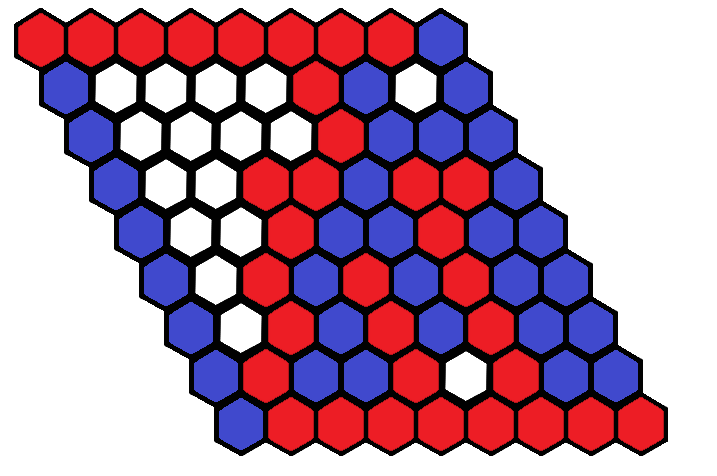
\includegraphics[width=1.1\linewidth]{./pictures/hexagonal_graphical_interface.png}
    \caption{figure}{L'interface graphique du jeu hex pour un plateaux lesenge de taille 8}
    \label{hex_board_h}
  \end{minipage}%
  \begin{minipage}{.5\textwidth}
    \centering
    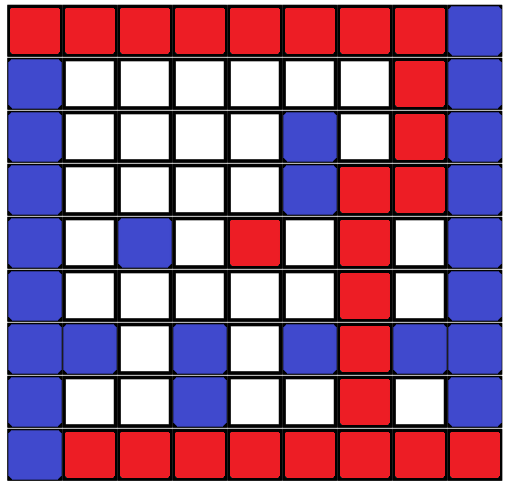
\includegraphics[width=.75\linewidth]{./pictures/squared_graphical_interface.png}
    \caption{figure}{L'interface graphique du jeu hex pour un plateaux carré de taille 8}
    \label{hex_board_c}
  \end{minipage}
\end{figure}

\subsection{\emph{Connex Player}}
Le second joueur que nous souhaitions implémenter est un joueur qui cherche à réduire la distance qui le sépare de l'autre bord du plateau. Il a la particularité de ne jamais accepter l'ouverture proposée par l'adversaire et tire son premier emplacement aléatoirement. C'est à partir de ce moment que la stratégie de réduire la distance séparant les deux bords intervient. Ce joueur calcule son plus court chemin reliant ses deux bords et le plus court chemin de son adversaire et choisit son coup de manière aléatoire dans l'intersection des deux plus courts, ce qui lui donne un aspect bloquant.
Pour faire cela, il faut tout d'abord savoir comment calculer un plus court chemin, ce qui va être expliqué dans les parties suivantes.

\subsubsection{Arbre des plus court chemins pondérés}
Afin de simplifier le calcule du plus court chemin, nous avons créé une structure \texttt{weighted\_tree (WTree)} où la valuation du graphe est stockée sous forme d'une matrice $m$ réelle. Cette valuation est initialisée au début du jeu par la fonction \texttt{init\_weights} soit par la méthode de \emph{Kirchhoff}(expliqué dans la partie \ref{part:kirch}) soit de la manière suivante :\\

Soit $V$ l'ensemble des sommets, et $E$ l'ensemble des arêtes du graphe de la table de jeu.\\
Soit $(i,j)\in V^2$
\begin{equation}
  m_{i,j} = \left\{
    \begin{array}{ll}
      v(i,j) \hspace{.5cm} si \hspace{.5cm} (i,j)\in E\\
      +\infty \hspace{.5cm} sinon
    \end{array}
  \right.
  \label{weights eq}
\end{equation}
avec:
\begin{align*}
  v \colon E &\longrightarrow \mathbb{R}\\
  \hspace{3cm}(x,y) &\longmapsto \left\{
    \begin{array}{ll}
      1 \quad\text{si x et y ne sont occupés par aucun joueur}\\
      0 \quad\text{si x et y sont de même couleur}\\
      0.5 \quad\text{si l'une de x et y est vide}\\
      +\infty \quad\text{sinon}
    \end{array}
  \right.
\end{align*}
La Figure \ref{fig:eval} illustre le fonctionnement de $v$ dans les quatre cas.\\
\begin{figure}[h!]
  \centering
  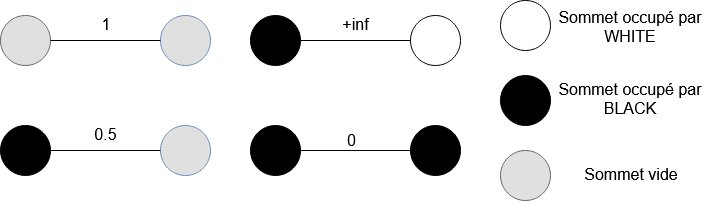
\includegraphics[width=.8\linewidth]{./pictures/edges_evaluation.PNG}
  \caption{Illustration de l'évaluation des arêtes}
  \label{fig:eval}
\end{figure}

La valuation est mise à jour après chaque coup par la fonction \texttt{update\_weights}. La valuation sert principalement à la construction de l'arbre des plus courts chemins. Il est modélisé par un tableau des prédécesseurs, ainsi qu'un tableau des distances entre le sommet de départ nommé \texttt{start} et un sommet quelconque qui a pour indice sa position sur le plateau.  Cela va donc permettre de construire le plus court chemin entre le sommet \texttt{start} et \texttt{end} qui correspondent aux bords du plateau. On crée un arbre vide pour chaque joueur avec la fonction \texttt{init\_tree} au début du jeu, ce qui initialise en même temps \texttt{start} et \texttt{end}.

L'étape suivante sera donc l'initialisation du tableau des prédécesseurs et du tableau des distances. Nous avons utilisé les algorithmes suivants pour cette initialisation.

\subsubsection{Algorithmes des plus courts chemins}
\label{p:short}
\paragraph{Algorithme de \emph{Dijkstra}}
L'algorithme de \emph{Dijkstra} est un algorithme de recherche de distance et de plus court chemin entre un sommet fixé (\texttt{start} dans notre cas) et tous les autres sommets d'un graphe à valuations positives. On initialise tout d'abord la distance de tous les sommets par la valeur $+\infty$ sauf \texttt{start} qui va être initialisée par $0$. Puis, on choisit un sommet $u$ parmi ceux qui n'ont pas encore été traités dont la distance à \texttt{start} est minimale. Pour chacun des successeurs $v$ de $u$, on compare $d(\texttt{start},v)$ avec $d(\texttt{start},u) + v(u,v)$ pour savoir s'il est judicieux de passer par $u$ pour arriver à $v$, dans ce cas, on met à jour le tableau des prédécesseurs avec $\texttt{pred}[v] = u$, et le tableau des distances par $\texttt{d}[v] = \texttt{d}[u] + v(u,v)$.

\begin{figure}[h!]
  \centering
  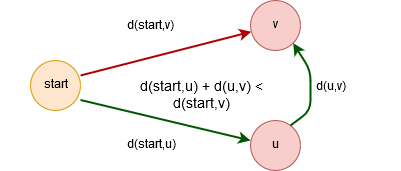
\includegraphics[scale=.7]{./pictures/Dijkstra.PNG}
  \caption{Passage par $u$ après la comparaison des distances}
  \label{fig:Dijkstra}
\end{figure}

Quand tous les successeurs de $u$ ont été examinés, on le rajoute à la liste des sommets traités $(\texttt{passed}[u] = 1)$, et l'on repart sur une nouvelle itération, jusqu'à passer sur tous les sommets.\\
La complexité de cet algorithme est de $O((n+m)log(n))$ où $n$ est le nombre des sommets et $m$ est le nombre des arêtes.

\paragraph{Algorithme de \emph{Bellman Ford}}
L'algorithme de \emph{Bellman Ford} est très similaire à celui de \emph{Dijktra}. La principale différence étant que, dans ce cas, les valuations peuvent être négatives.
L'initialisation va être la même que celle de \emph{Dijkstra}, mais la différence est qu'a chaque itération, on va traiter tous les sommets, puis on procède de la même manière que \emph{Dijkstra}.
Quand tous les successeurs du sommet $u$ ont été examinés, on passe à un autre sommet, mais toujours dans la même itération.
Une fois que tous les sommets ont été traités, on vérifie que lors de la dernière itération certaines valeurs des distances ont été mises à jour. Si c'est le cas, on repart sur une nouvelle itération, c'est-à-dire sur un traitement complet de tous les sommets. Sinon, l'algorithme est terminé.
Si un graphe ne contient pas de circuits absorbants, l'algorithme de \emph{Bellman Ford} se termine en au plus $n-1$ itérations. Ainsi, dans un graphe quelconque si l'algorithme continue à calculer des distances après $n-1$ itérations, ça veut dire que le graphe contient au moins un circuit absorbant, il suffit donc de rajouter une variable $k$ qui dénombre le nombre d'itérations.\\
Dans notre graphe, la valuation est positive, mais on aurait pu le pondérer par des valeurs négatives qui peuvent aider le joueur à choisir des chemins plus optimisés. La complexité de cet algorithme est polynomiale.

\paragraph{Algorithme de \emph{Floyd Warshall}}
Comme l'algorithme de \emph{Dijkstra}, celui-ci permet la recherche de plus court chemin, mais dans un graphe de valuation quelconque. Son avantage est le calcul des distances entre chaque pair de sommets.\\
Cet algorithme construit deux matrices \texttt{D} (matrice des distances) et \texttt{P} (matrice des prédécesseurs) qui seront remplies à l'aide de la relation de récurrence (\ref{eq:rec dist}).\\
Soit $(i,j)\in V^2$

\begin{equation}
  d(i,j,k) = \min(d(i,j,k-1), d(i,j,k-1) + d(k,j,k-1))\quad \text{pour $0\leq k\leq |V|-1$}
  \label{eq:rec dist}
\end{equation}

avec $\forall k\in[{0,\ldots,|V|-1]}\quad d(i,j,k)$ la longueur d'un plus court chemin d'origine $i$ et et d'extrémité $j$ en ne passant que par les sommets $1,2,\ldots,k$.\\
Pour l'initialisation, \emph{i.e} quand $k=0$, on a:\\

\begin{equation}
  d(i,j,0) = \left\{
    \begin{array}{ll}
      v(i,j) \quad \text{si $i$ et $j$ sont adjacents et $i\ne j$}\\
      0 \hspace{1.3cm} \text{si $i=j$}\\
      +\infty \hspace{.8cm} \text{sinon}
    \end{array}
  \right.
  \label{eq:rec dist init}
\end{equation}

La matrice \texttt{D} va être initialisée conformément à l'équation (\ref{eq:rec dist init}). La matrice \texttt{P} va être initialisée en attribuant $i$ à \texttt{P}$[i][j]$.\\
Notre but est de calculer $d(i,j,|V|-1)$ et la stocker dans \texttt{D}$[i][j]$. En effet, on procède en $|V|$ itérations, le calcule se faisant en utilisant la relation \eqref{eq:rec dist}. À la \emph{k-i\`eme} itération la valeur $d(i,j,k)$ est stockée dans \texttt{D}$[i][j]$ pour être utilisée dans l'itération suivante, et donc au bout des $|V|$ itérations la valeur de \texttt{D}$[i][j]$ sera bien celle cherchée.\\
Enfin, il suffit d'affecter la ligne \texttt{start} de \texttt{D} et de \texttt{P} respectivement aux tableaux \texttt{distance} et \texttt{pred}. La complexité de cet algorithme est de $O(|V|^3)$.

\subsubsection{Extraction du plus court chemin entre les deux bords}
Après avoir rempli le tableau \texttt{pred} en utilisant l'une des méthodes décrites précédemment, il suffit de remonter dans l'arbre des prédécesseurs depuis le sommet \texttt{end} en stockant les sommets dans la liste \texttt{path} jusqu'à arriver au sommet \texttt{start}. La figure \ref{fig:connex res} résume les étapes décrites ci-dessus.

\begin{figure}[h!]
  \centering
  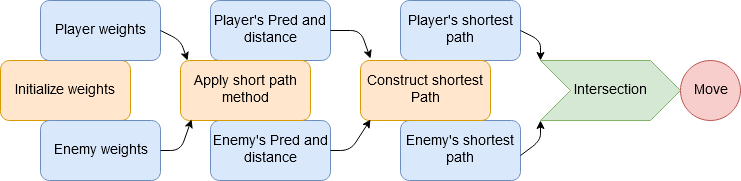
\includegraphics[width=.8\linewidth]{./pictures/Resume_connex.PNG}
  \caption{Résumé du fonctionnement du joueur \emph{Connex}}
  \label{fig:connex res}
\end{figure}

\subsubsection{Défauts de la stratégie}
Bien que cette stratégie permette au joueur de choisir un coup qui bloque l'adversaire et diminue la distance entre les deux bords du plateau, elle possède des défauts qui peuvent faire perdre le joueur, on trouve par exemple :
\begin{itemize}
\item Ne jamais accepter l'ouverture de l'adversaire peut amener à prendre un coup qui n'est pas bien placé.
\item De même choisir aléatoirement l'ouverture peut amener à choisir un coup qui n'est pas bien placé.
\item Un plateau du jeu n'a pas forcément un seul plus court chemin, donc l'intersection des plus courts chemins n'est pas forcément un blocage, il se peut que l'adversaire choisisse un autre plus court chemin.
\end{itemize}

\subsection{\emph{Minimax Player}}
Nous avons pensé à corriger les défauts du joueur \emph{Connex} en utilisant un algorithme qui cherche à minimiser les pertes en considérant que l'adversaire joue d'une manière optimale.
Le coup choisi par cette stratégie dépend principalement de la fonction d'évaluation du plateau. La fonction que nous avons choisie est une fonction gloutonne, qui consiste à calculer la différence des distances (du joueur et de son adversaire) restantes pour relier les bords du plateau.

\subsubsection{Explication de la stratégie}
La stratégie construit une partie virtuelle du jeu où les joueurs sont le \texttt{MIN} et le \texttt{MAX}. Le but du joueur \texttt{MAX} est de maximiser le score donné par l'heuristique, et le contraire pour le \texttt{MIN} (dans notre cas le \texttt{MAX} est le \texttt{player} et le \texttt{MIN} est l'\texttt{Enemy}), en suivant ces étapes :
\begin{itemize}
\item Créer un graphe pondéré temporaire pour chaque coup choisi, puis appeler la fonction \texttt{minimax} qui va générer un arbre du jeu.
\item Chercher le plus court chemin des deux joueurs.
\item Si on maximise, on copie l'ancien graphe et on remplit cette copie par le coup choisi parmi les sommets du plus cours chemin du \texttt{Player}. Ensuite, on fait un appel récursif de la fonction \texttt{minimax} qui crée un sous-arbre dans lequel on va minimiser. Enfin, on retourne le maximum des scores des coups choisis.
\item On fait la même chose en cas de minimisation, la différence est dans le choix du coup dans le plus court chemin de l'\texttt{Enemy}, et on retourne le minimum au lieu du maximum des scores.
\item Ce processus s'arrête quand la hauteur de l'arbre atteint la valeur prédéfinie, dans ce cas, on renvoie la valeur heuristique du sommet choisi qui est la différence des distances des plus courts chemins obtenus en choisissant ce sommet.
\item Enfin, le joueur choisit le coup ayant le plus grand score s'il n'est pas déjà occupé sinon il choisit aléatoirement dans l'ensemble des sommets disponibles.
\end{itemize}
La construction des plus courts chemins utilisées dans la stratégie suit les étapes décrites dans la partie \ref{p:short}.\\
L'algorithme \texttt{minimax} utilisé est optimisé par une méthode nommée \emph{Alpha-Beta} qui diminue le nombre des sommets évalués en éliminant des branches inutiles de l'arbre du jeu.\\
On peut aussi utilisé l'heuristique de \emph{Kirchhoff} pour une meilleure évaluation.\\

\subsubsection{Défaut de la stratégie}
La complexité de cette stratégie est exponentielle, alors le joueur prend beaucoup de temps en choisissant un coup, ce qui rend le jeu impossible pour des plateaux de taille très grande. La diminution des sommets évalués dans les deux phases de \texttt{minimax} (évaluation des sommets du plus court chemin) n'impacte pas d'une façon remarquable sur le temps d'exécution.\\

\subsection{Heuristique de Kirchhoff}
\label{part:kirch}
Dans le but de développer encore des nouvelles stratégies de joueurs, nous avons étudié une stratégie expliquée par Anshelevich dans l'article ``The Game of Hex: An Automatic Theorem Proving Approach to Game Programming''.

Cette stratégie utilise les différentes lois de Kirchhoff (d'où son nom) pour calculer les plateaux les plus favorables à un joueur. Pour un joueur donné, on considère un circuit électrique reliant les deux bords de la même couleur que celle du joueur et passant par le plateau. Ensuite, on attribue à chacune des cases du plateau une valeur qui correspond à sa résistance. Ainsi pour le joueur de couleur $A$, la résistance $R_A$ d'un emplacement est donné par les équations (\ref{eq:res}) ci-dessous.

\begin{equation}
  R_A = \left \{
    \begin{array}{c l}
      0 & \text{si la case est de la couleur du joueur $A$}\\
      +\infty & \text{si la case est de la couleur de l'adversaire}\\
      1 & \text{sinon}\\
    \end{array}
  \right.
  \label{eq:res}
\end{equation}

\begin{figure}[h]
  \centering
  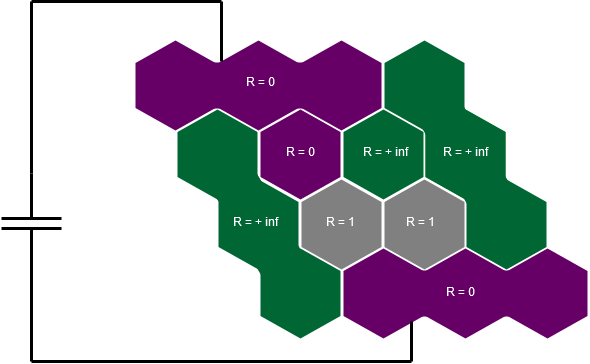
\includegraphics[width=.8\linewidth]{./pictures/kirchoff.png}
  \caption{Représentation d'un plateau de jeu hexagonal de largeur 3. Les résistances sont attribuées en considérant le joueur violet.}
  \label{fig:kirch}
\end{figure}

En considérant le plateau de la manière présenté ci-dessus et dans la figure \ref{fig:kirch}, il est possible d'évaluer la résistance du plateau. Plus la résistance est élevée, moins le plateau est à l'avantage du joueur. En calculant plusieurs plateaux différents, il est possible de mettre en place un algorithme qui privilégiera toujours celui ayant le moins de résistance. Mais il est également possible d'utiliser des algorithmes plus complexes qui se servent du calcul de la résistance d'un plateau. Un programme pourrait être capable d'apprendre les mouvements des joueurs auxquels il est confronté, lui permettant ainsi de prévoir plusieurs coups à l'avance, le plateau le plus favorable.

Malheureusement, cette stratégie n'a finalement pas été implémentée par manque de temps.
\section{Critiques}
Le projet s'est, dans l'ensemble, très bien déroulé. Mais il est tout de même nécessaire d'évoquer les situations plus difficiles qui ont été rencontrées.

\subsection{Manque de maîtrise du Kanban}
L'une des critiques majeures qu'il est possible de faire sur le déroulement du développement, est l'utilisation du tableau Kanban. Il y avait parfois un manque de transparence sur les activités en cours de réalisation. Cela couplé avec les difficultés de communications liées à l'éloignement, provoquait parfois des problèmes divers. Par exemple des conflits lors d'une fusion de branches car un fonctionnement a été réalisé sans être indiqué. Cela a aussi pu faire déboucher sur une répartition des tâches moins égalitaire.

\subsection{Manque de documentation}
La documentation à été largement délaissée par certains lors de l'écriture du code. Il y a eu des phases entières dédiées à l'écriture de la documentation, ce qui devient plus une corvée pour celui qui la réalise. Or, la documentation est très importante pour la compréhension du code, par les autres membres de l'équipe, mais également pour des membres extérieurs. Une écriture systématique de la documentation au préalable de l'écriture d'une nouvelle fonction nous aurait fait facilement gagner du temps.

\section{Conclusion}
Malgré de nombreux points améliorables tant au niveau du code que de l'organisation, ce projet a été très enrichissant. Il nous a permis d'utiliser des pratiques de programmations étudiées lors des différents cours, de résoudre des problèmes en utilisant nos connaissances ainsi que de nous mettre à l'épreuve notamment avec une communication plus compliquée qu'a l'habitude.

\end{document}
